\documentclass[pdftex,ptm,12pt,a4paper]{report}
\renewcommand{\baselinestretch}{1.5}
\setcounter{secnumdepth}{5}

% PDF search & cut'n'paste
\usepackage{cmap}
\usepackage[table,xcdraw]{xcolor}

% Cyrillic support
\usepackage{mathtext}
\usepackage{amsmath}
\usepackage[T1,T2A]{fontenc}
\DeclareSymbolFont{T2Aletters}{T2A}{cmr}{m}{it}
\usepackage[utf8]{inputenc}
\usepackage{multicol}

\usepackage[bottom=20mm,top=20mm,right=20mm,left=30mm,headsep=0cm,nofoot]{geometry}

\usepackage{array}
\newcolumntype{C}[1]{>{\centering\let\newline\\\arraybackslash\hspace{0pt}}m{#1}}

\makeatletter
\renewcommand*{\ps@plain}{%
  \let\@mkboth\@gobbletwo
  \let\@oddhead\@empty
  \def\@oddfoot{%
    \reset@font
    \hfil
    \thepage
    % \hfil % removed for aligning to the right
  }%
  \let\@evenhead\@empty
  \let\@evenfoot\@oddfoot
}
\makeatother
\pagestyle{plain}

\usepackage[pdftex]{graphicx}
\usepackage{caption}
\usepackage{subcaption}
\usepackage[russian,english]{babel}
    \addto{\captionsenglish}{\renewcommand{\bibname}{Литература}}
    \addto\captionsenglish{\renewcommand{\figurename}{Рис.}}
    \addto\captionsenglish{\renewcommand{\contentsname}{Содержание}}
    \addto\captionsenglish{\renewcommand{\proofname}{Доказательство}}
\usepackage{hyperref}
\usepackage{url}
\usepackage{abstract}
\usepackage{float}
\usepackage{amsthm}
\usepackage{amssymb}
\usepackage{amsmath}
\renewcommand*{\proofname}{Доказательство}
\usepackage{indentfirst}
\usepackage{color}
\usepackage{natbib}
\usepackage{bbm, dsfont}


% Detect whether PDFLaTeX is in use
\usepackage{ifpdf}

% Fix links to floats
\usepackage[all]{hypcap}

\makeatletter
\renewcommand{\@chapapp}{Часть}
\makeatother

% Theorem Styles
\newtheorem{theorem}{Теорема}[chapter]
\newtheorem{lemma}[theorem]{Лемма}
\newtheorem{claim}[theorem]{Теорема}
% Definition Styles
\theoremstyle{definition}
\newtheorem{definition}{Определение}[chapter]
\newtheorem{example}{Пример}[chapter]
% Rule for Title Page
\newcommand{\HRule}{\rule{\linewidth}{0.5mm}}

\begin{document}

\begin{titlepage}
\newpage

\begin{center}
МИНИСТЕРСТВО ОБРАЗОВАНИЯ И НАУКИ РОССИЙСКОЙ ФЕДЕРАЦИИ \\
\vspace{0.5cm}
ГОСУДАРСТВЕННОЕ ОБРАЗОВАТЕЛЬНОЕ УЧРЕЖДЕНИЕ \\*
ВЫСШЕГО ПРОФЕССИОНАЛЬНОГО ОБРАЗОВАНИЯ\\*
"МОСКОВСКИЙ ФИЗИКО-ТЕХНИЧЕСКИЙ ИНСТИТУТ \\*
(ГОСУДАРСТВЕННЫЙ УНИВЕРСИТЕТ)" \\*
\vspace{0.5cm}
ФАКУЛЬТЕТ ИННОВАЦИЙ И ВЫСОКИХ ТЕХНОЛОГИЙ \\*
КАФЕДРА АНАЛИЗА ДАННЫХ \\*
\hrulefill
\end{center}


\vspace{8em}

\begin{center}
\Large Выпускная квалификационная работа по направлению 01.03.02 <<Прикладные математика и информатика>> \linebreak НА ТЕМУ:
\end{center}

\vspace{2.5em}

\begin{center}
\textsc{\large{\textbf{НЕЙРОСЕТЕВЫЕ МОДЕЛИ В ЗАДАЧАХ ИНТЕРПРЕТАЦИИ ДАННЫХ ФМРТ ПРИ АУДИАЛЬНОЙ СТИМУЛЯЦИИ}}}
\end{center}

\vspace{6.5em}

\begin{flushleft}
Студент \hrulefill Медведева А.Е. \\
\vspace{1.5em}
Научный руководитель к.ф-м.н \hrulefill Артемов А.В.\\
\vspace{1.5em}
Зам. зав. кафедрой д.ф-м.н, профессор \hrulefill Бунина Е.И.
\end{flushleft}

\vspace{\fill}

\begin{center}
МОСКВА, 2017
\end{center}

\end{titlepage}

\tableofcontents

\sloppy

%\chapter{Введение}

\chapter{Общая постановка эксперимента}
\section{ФМРТ в измерении активности мозга}

Функциональная магнитно-резонансная томография, или ФМРТ, - это метод измерения активности головного мозга. Он работает путем обнаружения изменений насыщения крови кислородом, а также потоков крови, возникающих в ответ на нейронную активность. Когда зона мозга более активна, она потребляет больше кислорода, и чтобы удовлетворить этот растущий спрос, увеличивается приток крови к рабочей области. ФМРТ может быть использована для создания карт активности, показывающих, какие части мозга вовлечены в конкретный психический процесс.

Каждое ФМРТ измерение -- последовательность трехмерных сканов мозга, где каждый скан есть набор значений сигнала на каждом маленьком участке мозга, называемым вокселем и представляющим собой параллелепипед с сторонами порядка нескольких милиметров (см. \ref{fmri_result}).

\begin{figure}[h]
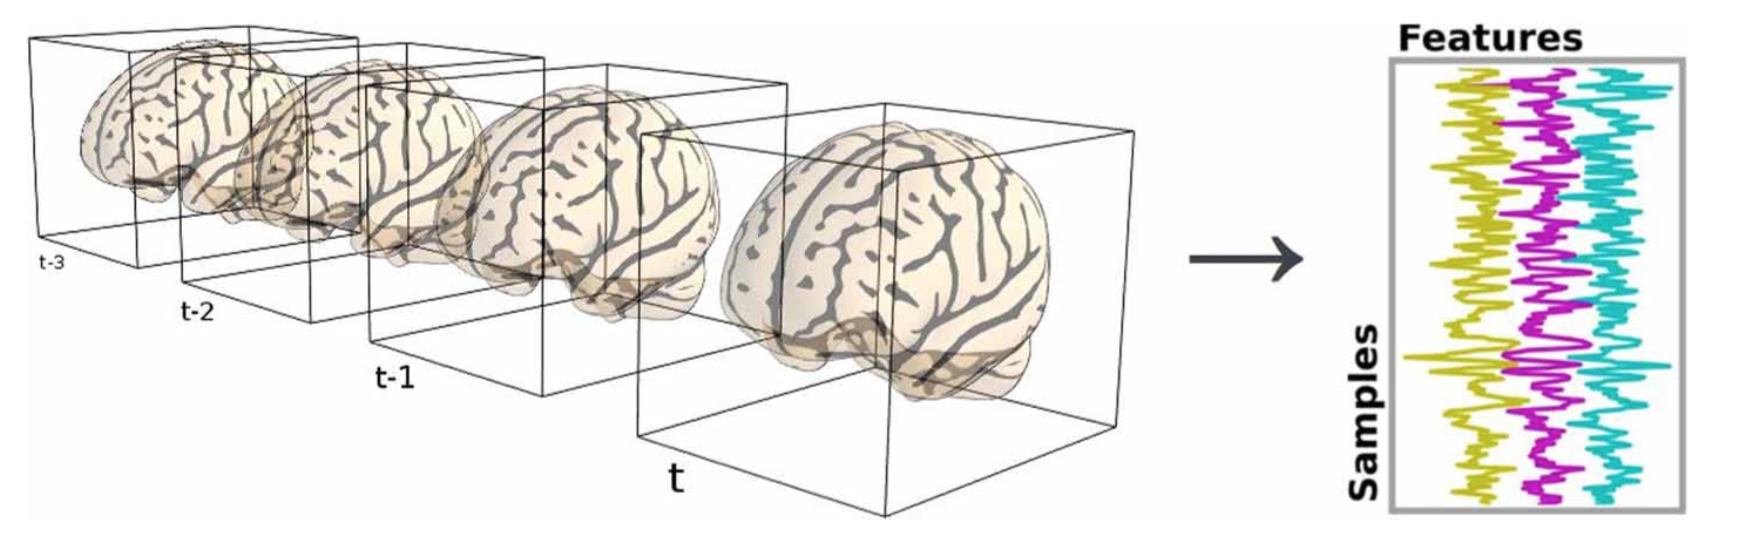
\includegraphics[scale=0.2]{images/fmrt_result.png}
\centering
\caption{ФМРТ измерение.}
\label{fmri_result}
\end{figure}

ФМРТ имеет несколько преимуществ перед другими методами измерения мозговой активности:
\begin{enumerate}
\item Этот метод является неинвазивным и не использует рентгеновское излучение, что делает его безопасным для человека.

\item Имеет хорошую пространственно-временное разрешение. На рисунке \ref{fmri} показано сравнение ФМРТ с другими методами измерения активности мозга, такими как энцефалография(МЭГ, ЭЭГ) и позитронно-эмисионная томография (ПЭТ).

\begin{figure}[h]
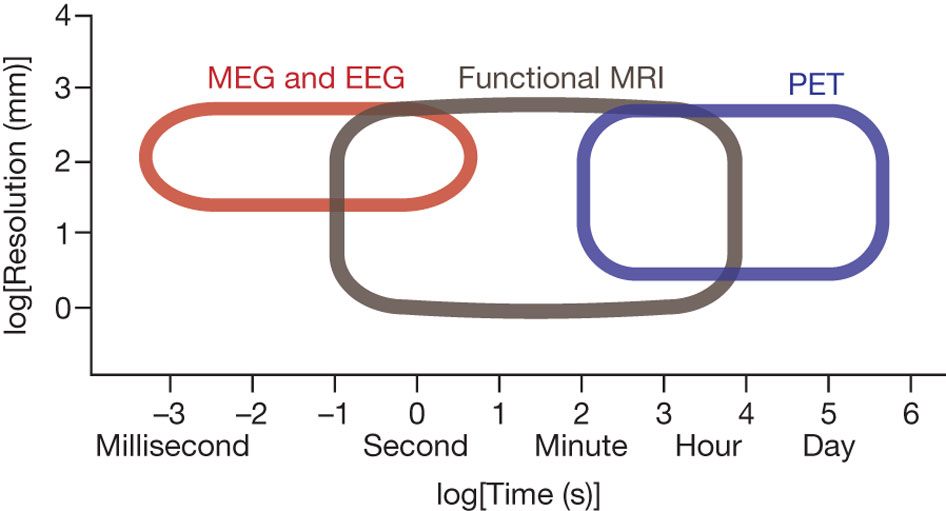
\includegraphics[scale=0.3]{images/fmrt.jpg}
\centering
\caption{Сравнение ФМРТ, ПЭТ и МЭГ.}
\label{fmri}
\end{figure}

\item Его легко использовать для постановки экспериментов.
\end{enumerate}

Из недостатков можно выделить следующие:

\begin{enumerate}
\item Для точного измерения необходимо, чтобы человек оставался неподвижным. Движения головы, вызванные биением сердца, дыханием и  ерзаньем, являются одним из основных источников шума.

\item Наличие шума, вызванного неоднородностью магнитного поля, используемого для измерения.

\item ФМРТ измеряет уровень активности не напрямую, а косвенно.

\item Уровень насыщения крови кислородом, который измеряет ФМРТ, изменяется очень медленно. Его изменение происходит с некоторой задержкой (обычно порядка пары секунд), так как необходимо некоторое время для сосудистой системы в ответ на потребность мозга в глюкозе. После чего он обычно поднимается до пика примерно через 5 секунд после стимула. Если нейроны остаются активными, пик распространяется на плоское плато. После остановки деятельности, сигнал падает ниже исходного уровня -- явление, называемое недолетом. С течением времени сигнал восстанавливается до базовой линии (см. \ref{hrf}). 

\begin{figure}[h]
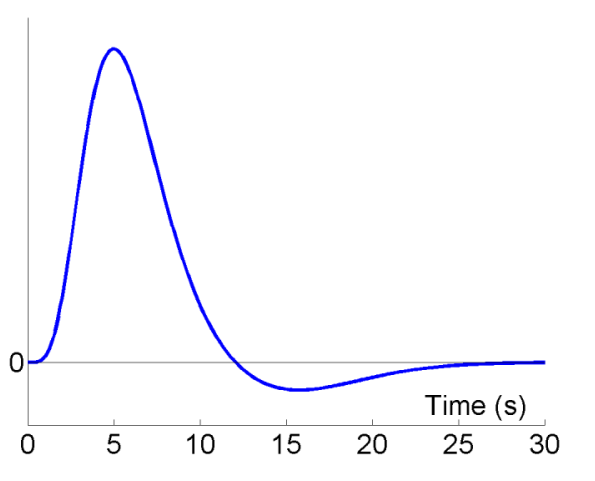
\includegraphics[scale=0.4]{images/hrf.png}
\centering
\caption{Уровень насыщения крови в зависимости от времени.}
\label{hrf}
\end{figure}

\end{enumerate}

\section{Постановка задачи}

В типичном эксперименте с помощью ФМРТ по внешнему стимулу строится матрица признаков $\textbf{X}.$ Например, при аудиальной стимуляции строки матрицы $\textbf{X}$ -- векторы, соответствующие словам из текста аудио. Измерения ФМРТ -- матрица ответов $\textbf{Y},$ столбцы которой соотвествуют вокселям, строки -- вектор активации мозга в конкретный момент времени. Далее задача сводится к построению модели $f,$ максимизирующую коррелюцию Пирсона на тестовой выборке:
$$Pirson(\textbf{Y}_{test},\ f(\textbf{X}_{test})) \rightarrow max_{f}.$$

В случае, если для каждого вокселя своя модель из класса $\mathcal{F}$, то максимизируется средняя корреляция по вокселям. Обозначим число вокселей за $N$, $i$--ый столбец матрицы $\textbf{Y}$ за $\textbf{Y}^{;,i}$. Тогда функционал для максимизации выглядит следующим образом:

$$\frac{1}{N} \sum_{i=1}^{N} Pirson(\textbf{Y}_{test}^{:,i}, f_{i}(\textbf{X}_{test})) \rightarrow max_{\mathcal{F}}.$$


\chapter{Обзор литературы}
\section{Семантический атлас мозга}\label{complex}


Работа \cite{huth2016natural} группы американский нейробиологов посвящена созданию семантического атласа мозга на основе данных, полученных с помощью ФМРТ. Ученым удалось выделить области на фронтальной коре, ответственные за конкретные семантический группы, такие как социальные явления, абстрактные понятия, количественные слова. 

\begin{figure}[h]
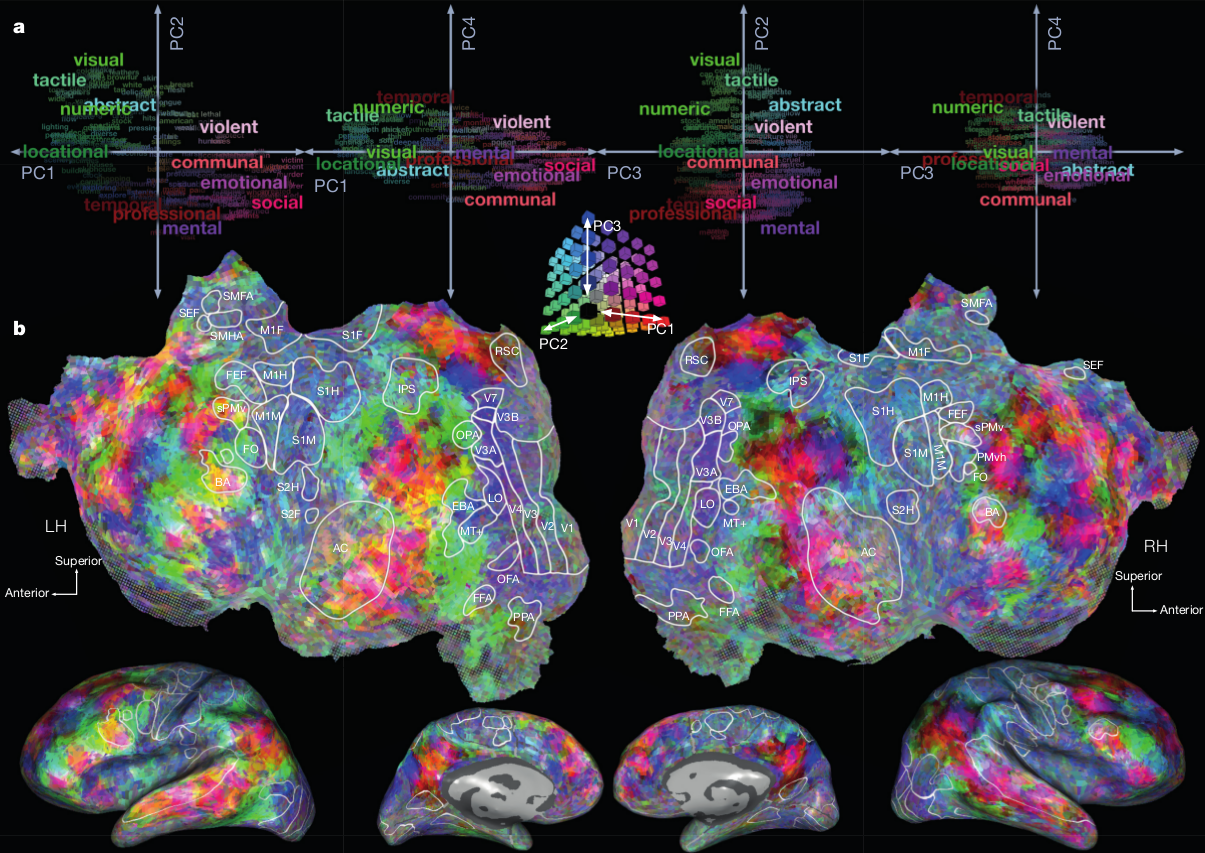
\includegraphics[scale=0.4]{images/galant_results.png}
\centering
\caption{Результаты из работы \cite{huth2016natural}.}
\label{huth_result}
\end{figure}

\begin{figure}[h]
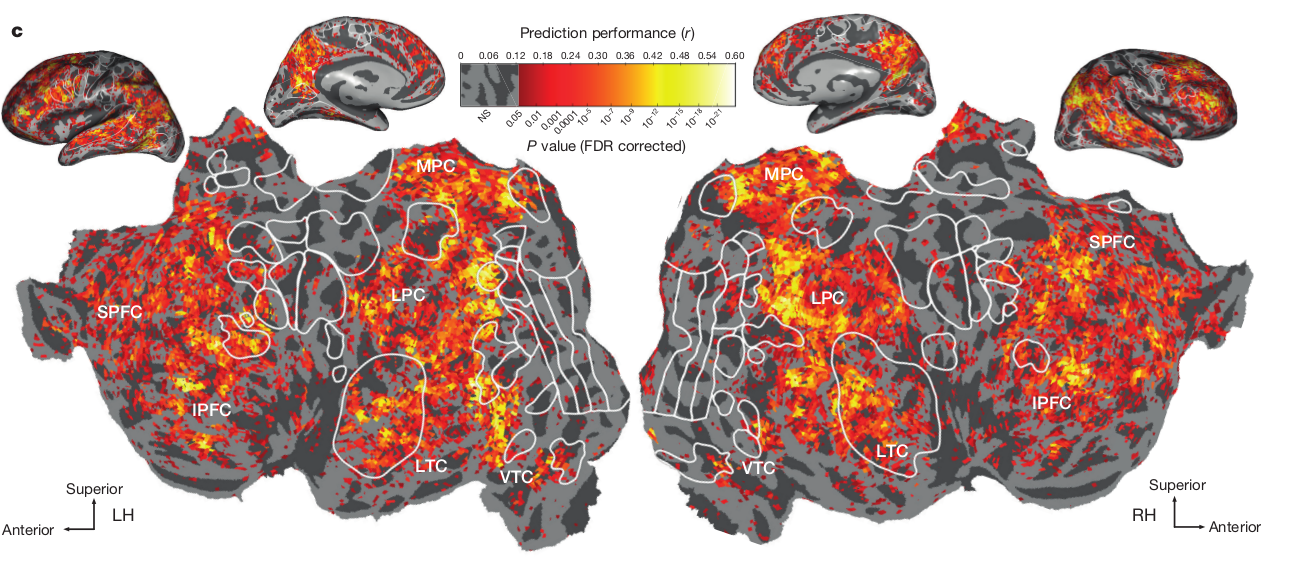
\includegraphics[scale=0.4]{images/map_result_huth.png}
\centering
\caption{Результаты из работы \cite{huth2016natural}.}
\label{map_huth_result}
\end{figure}

Эксперимент был построен следующим образом: 8 испытуемых слушали 2 часа рассказы из радиопередачи. После чего авторы подсчитали на большом корпусе матрицу совместной встречаемости каждого слова из текста аудио и 985 самых частоупотребимых английских слов. Каждая строка этой матрицы соответствовала представлению слова из аудио в 985-мерном пространстве. Для установления зависимости между признаками аудиостимула (представления слов из аудио) и измерениями ФМРТ авторы использовали гребневую регрессию. Далее изучались вектора весов регрессии, соответствующей каждому вокселю, для чего они были спроектированы в четырехмерное пространство с помощью метода главных компонент. В это же пространство были спроектированы и слова из аудиостимула. С помощью алгоритма k средних спроецированные слова были сгруппированы в 12 категорий. После чего авторы раскрасили пространство из первых трех главных векторов и визуализировали результат (см. \ref{huth_result}). 

Интересна проекция на первую компоненту: положительные знак имеют слова, относящиеся к человеку и человеческим взаимодействиям, отрицательную -- описания восприятия, местоположения, количества. На рис. \ref{map_huth_result} показана средняя корееляция Пирсона в проекции на поверхность долей. Видно, что зоны LTC, VTC, LPC, MPC, SPFC и IPFC предсказываются достаточно хорошо (корреляция значимо больше нуля), ранее эти зоны считались семантической системой мозга.


\section{Применение нейросетевых методов}

\begin{figure}[h]
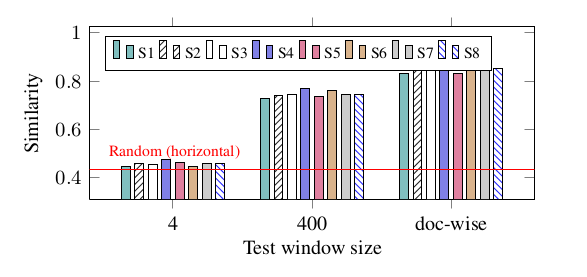
\includegraphics[scale=0.7]{images/neural_nets.png}
\centering
\caption{Результаты из работы \cite{qian2016bridging}.}
\label{qian_res}
\end{figure}

В статье \cite{qian2016bridging} изучалось предсказательная способность LSTM юнитов в зависимости от архитектуры (наличия гейтов). В качестве данных авторы использовали активацию мозга в процессе чтения главы из книги "Гарри Поттер". Эксперимент был устроен следующим образом: авторы обучили нейронную сеть предсказывать следующее слово в тексте на оставшихся главах. Далее с помощью метода наименьших квадратов устанавливалась зависимость между вектором внутреннего состояния нейросети в момент предсказывания следующего слова и вектором активации всего мозга перед прочтением этого слова. В качестве меры качества модели авторы использовали косинусное расстояние между предсказанием и дейсвительной активацией мозга, нормализованным на отрезок [0,1]. Несмотря на то, что статья была посвящена изучению LSTM юнитов, авторы получили неплохую предсказательную способность (см. \ref{qian_res}), максимальное качество 0.86 достигалось при максимальном окне просмотра на тесте и использовании вектора внутренней памяти сети.


\chapter{Эксперимент}

\section{Описание данных}

Данные были взяты с открытой базы данных ФМРТ openfmri.org. В ходе эксперимента 20 участников в возрасте от 21 до 38 лет 2 часа (8 сегментов по 15 минут) слушали немецкую версию аудиофильма "Форрест Гамп". При этом ФМРТ сканер измерял каждые две секунды мозговую активность с пространственным разрешением $2.75\ mm^3$.

\section{Препроцессинг данных}

К данным ФМРТ была применена коррекция движений а также подавление шума с помощью библиотеки FLIRT, далее ФМРТ сигнал был посегментно нормализан, чтобы иметь среднее ноль и дисперсию 1. 

Для создания транскрипции использовался инструмент Google Api Speech Recognition. Далее транскрипция была пословесно выровнена с помощью библиотеки aeneas, после чего с помощью предобученной модели word to vec слова из транскрипции были переведены в трехсотмерные вектора из $\mathbb{R}^{300}.$ Затем полученные представления слов интерполировались с ядром Ланшица, чтобы согласовать моменты произношения слов и моменты измерения ФМРТ. Ввиду того что отклик конкретного вокселя происходит с некоторой задержкой, а также ввиду сложной формы сигнала отклика (\ref{hrf}), для каждого момента измерения стимул, соответствующий этому моменту был сконкатенирован с тремя предыдущими. Таким образом получилось 1200 семантических признаков. Далее из 3600 пар стимул - измерение первые 3100 использовались для обучения и последние 500 для валидации.


\section{Линейные методы}

Повторяя эксперимент авторов статьи \citep{huth2016natural}, мы использовали повоксельно гребнеую регрессию для предсказания ФМРТ отклика.

\begin{figure}[h]
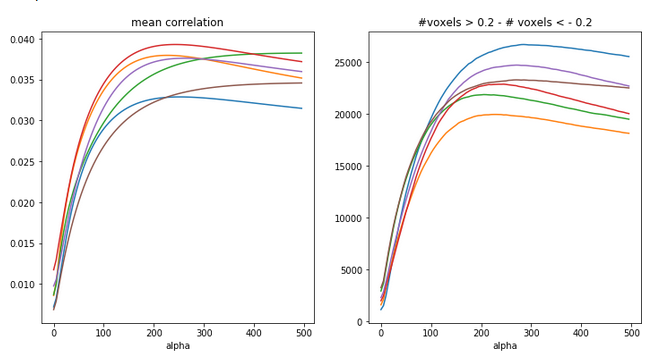
\includegraphics[scale=0.6]{graphics/correlations2.png}
\centering
\caption{Корреляция на тесте в зависимости от параметра $\alpha$ }
\label{corr_many}
\end{figure}

На рисунке \ref{corr_many} показаны результататы корреляции на тесте в зависимости от параметра регулязации альфа гребневой регрессии для 6 человек. На первом графикепоказана средняя повоксельная корреляция, на втором -- разница числа вокселей, корреляция которых больше 0.2 и числа вокселей, корреляция которых меньше -0.2.

Видно, что альфы примерно одного порядка и средняя корреляция стаильно больше нуля. На рисунке \ref{sub3_hist} показана гистограмма корреляций вокселей для третьего испытуемого. Видно, что положительных значений больше и среднее значимо отличается от нуля. Критерии согласия Колмогорова для проверки на нормальность показывает p-value равным 0, что означает что данное распределение нельзя считать нормальным. Также критерий Вилконсона для проверки на симметричность относительно нуля также дает p-value равным 0.

\begin{figure}[h]
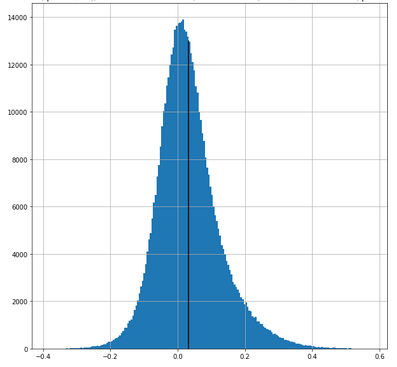
\includegraphics[scale=0.6]{graphics/sub3_prep2.png}
\centering
\caption{Гистограмма корреляций при $\alpha=245$.}
\label{sub3_hist}
\end{figure}

На рисунке \ref{sub3_bv} показан типичный сигнал ФМРТ и его предсказание, нормализованные для наглядности. Выведем срезы мозга  по оси z -- видим, что хорошо предсказывается височные доли (корреляция достигает 0.4 для всех субъектов), которые отвечают за слух и ассоциативное мышление. На рисунке\ref{slices} показаны срезы для этих зон для четырех субъектов. Видно, что зоны активации приблизительно повторяют друг друга, на рисунке \ref{huth_result} эти зоны больше всего реагируют на слова из социальной группы. 

\begin{figure}[h]
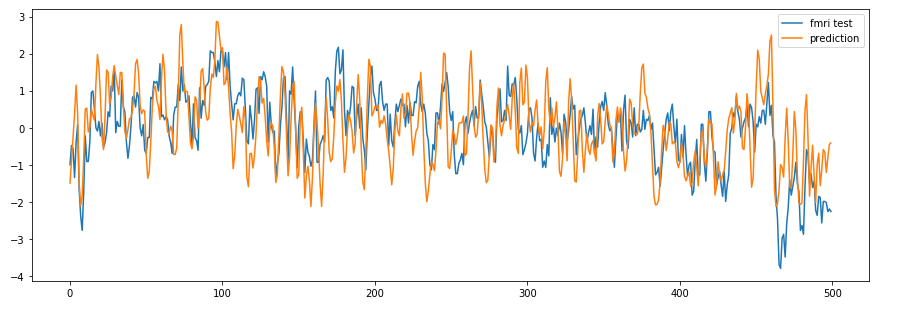
\includegraphics[scale=0.5]{graphics/sub3_prep2_bestvoxel.png}
\centering
\caption{Отклик вокселя и его предсказание.}
\label{sub3_bv}
\end{figure}

\begin{figure}[h]
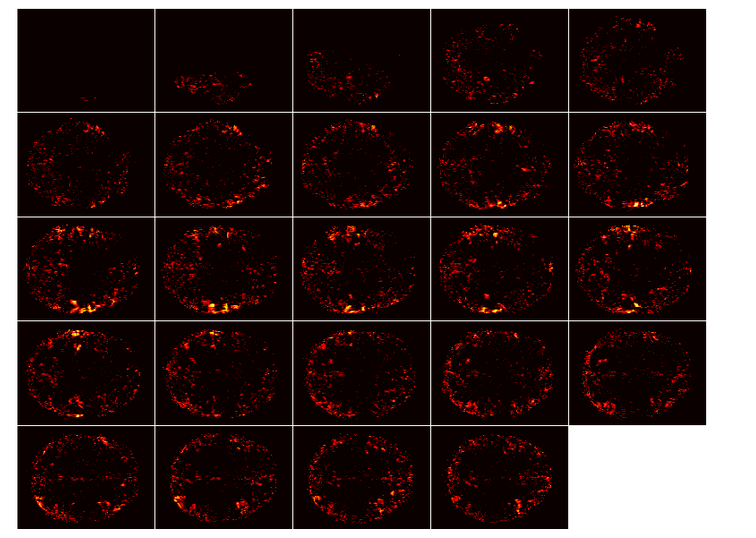
\includegraphics[scale=0.65]{graphics/sub12_trunk01.png}
\includegraphics[scale=0.4]{images/colorbar.png}
\centering
\caption{Значимые результаты предсказания (корреляция > 0.1) для 12-ого субъекта.}
\label{sub12_mosaic}
\end{figure}

\begin{figure}[h]
\begin{multicols}{4}
\centering
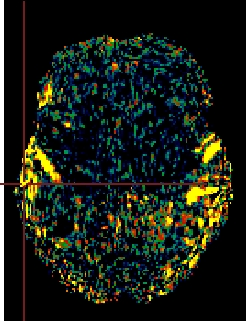
\includegraphics[scale=0.5]{graphics/slices/sub3.png}
\centering
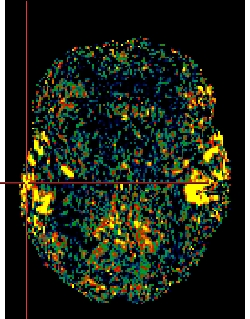
\includegraphics[scale=0.51]{graphics/slices/sub6.png}
\hfill
\centering
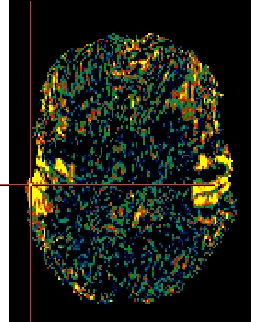
\includegraphics[scale=0.5]{graphics/slices/sub9.png}
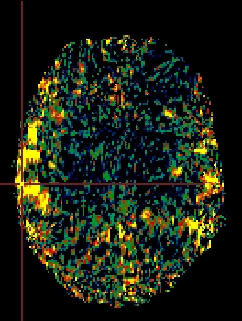
\includegraphics[scale=0.5]{graphics/slices/sub12.png}
\hfill
\centering
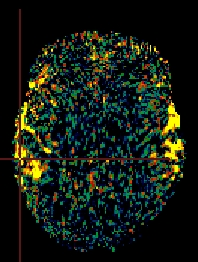
\includegraphics[scale=0.61]{graphics/slices/sub14.png}
\centering
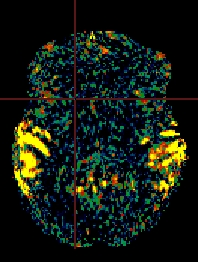
\includegraphics[scale=0.61]{graphics/slices/sub15.png}
\hfill
\includegraphics[scale=0.65]{graphics/slices/colorbar.png}
\label{slices}
\end{multicols}
\centering
\caption{Карта корреляции ФМРТ отклика и предсказания.}
\end{figure}


\section{Нейросетевые методы и планы на будущее}
Планируется провести анализ весов, полученных в гребневой регрессии, а также попробовать рекуррентные нейронные сети для предсказания активности мозга.

\bibliography{diplomnaya_rabota}
\bibliographystyle{plain}

\end{document}






